%% LyX 1.6.3 created this file.  For more info, see http://www.lyx.org/.
%% Do not edit unless you really know what you are doing.
\documentclass[ngerman]{beamer}
\usepackage[T1]{fontenc}
\usepackage[latin9]{inputenc}
\setcounter{secnumdepth}{3}
\setcounter{tocdepth}{3}
\usepackage{babel}

\usepackage{float}
\usepackage{graphicx}
\hypersetup{unicode=true, pdfusetitle,
 bookmarks=true,bookmarksnumbered=true,bookmarksopen=false,
 breaklinks=false,pdfborder={0 0 0},backref=false,colorlinks=false,}
 
\makeatletter
%%%%%%%%%%%%%%%%%%%%%%%%%%%%%% Textclass specific LaTeX commands.
 % this default might be overridden by plain title style
 \newcommand\makebeamertitle{\frame{\maketitle}}%
 \AtBeginDocument{
   \let\origtableofcontents=\tableofcontents
   \def\tableofcontents{\@ifnextchar[{\origtableofcontents}{\gobbletableofcontents}}
   \def\gobbletableofcontents#1{\origtableofcontents}
 }
 \makeatletter
 \long\def\lyxframe#1{\@lyxframe#1\@lyxframestop}%
 \def\@lyxframe{\@ifnextchar<{\@@lyxframe}{\@@lyxframe<*>}}%
 \def\@@lyxframe<#1>{\@ifnextchar[{\@@@lyxframe<#1>}{\@@@lyxframe<#1>[]}}
 \def\@@@lyxframe<#1>[{\@ifnextchar<{\@@@@@lyxframe<#1>[}{\@@@@lyxframe<#1>[<*>][}}
 \def\@@@@@lyxframe<#1>[#2]{\@ifnextchar[{\@@@@lyxframe<#1>[#2]}{\@@@@lyxframe<#1>[#2][]}}
 \long\def\@@@@lyxframe<#1>[#2][#3]#4\@lyxframestop#5\lyxframeend{%
   \frame<#1>[#2][#3]{\frametitle{#4}#5}}
 \makeatother
 \def\lyxframeend{} % In case there is a superfluous frame end

\makeatother

\begin{document}

\title{Wochenbericht}


\author{Max Mustermann}


\institute{Studienprojekt A: SIMPL}


\date{12. November 2009}


\titlegraphic{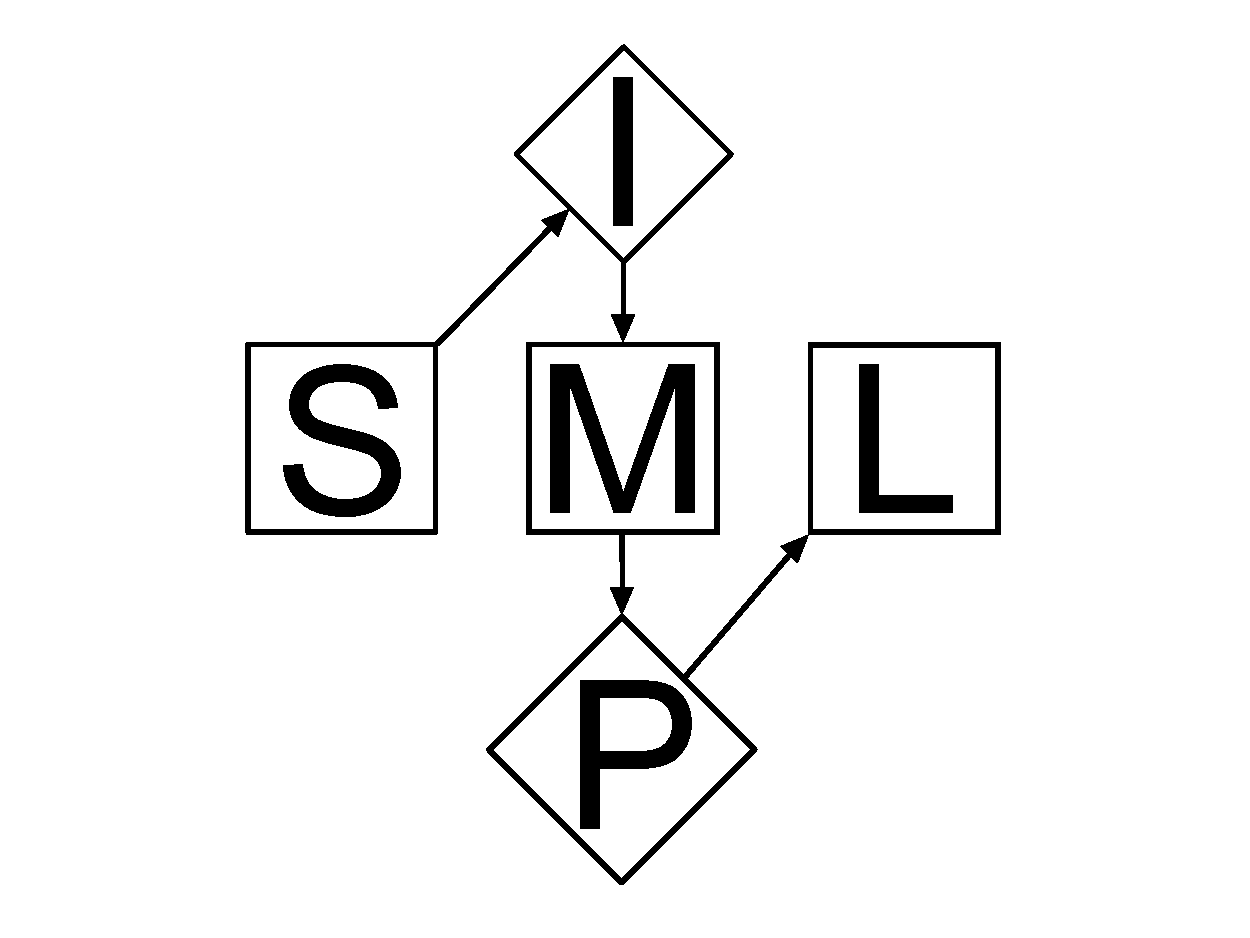
\includegraphics[scale=0.2]{SIMPL}}

\makebeamertitle

\lyxframeend{}\section*{Outline}


\lyxframeend{}\lyxframe{}

\tableofcontents{}


\lyxframeend{}


\lyxframeend{}\section{Geplante Aufgaben und T�tigkeiten}


\lyxframeend{}\lyxframe{Geplante Aufgaben und T�tigkeiten}
\begin{enumerate}
\item aufgaben
\end{enumerate}

\lyxframeend{}


\lyxframeend{}\section{Erledigte Aufgaben und T�tigkeiten}


\lyxframeend{}\subsection{�bersicht}


\lyxframeend{}\lyxframe{Erledigte Aufgaben und T�tigkeiten}


\framesubtitle{�bersicht}
\begin{enumerate}
\item aufgaben
\end{enumerate}

\lyxframeend{}


\lyxframeend{}\subsection{Ben�tigte Arbeitszeit/Aufw�nde}


\lyxframeend{}\lyxframe{Erledigte Aufgaben und T�tigkeiten}


\framesubtitle{Investierte Arbeitszeit/Aufw�nde}
\begin{enumerate}
\item aufw�nde
\end{enumerate}

\lyxframeend{}


\lyxframeend{}\section{Gewonnene Erkenntnisse}


\lyxframeend{}\lyxframe{Gewonnene Erkenntnisse}
\begin{itemize}
\item erkenntnisse
\end{itemize}

\lyxframeend{}


\lyxframeend{}\section{Neues f�r SIMPL}


\lyxframeend{}\lyxframe{Neues f�r SIMPL}

\begin{center}
Diagramme, Screenshots, usw.
\par\end{center}


\lyxframeend{}


\lyxframeend{}\section{Verwendete Quellen/Literatur}


\lyxframeend{}\lyxframe{Verwendete Quellen/Literatur}
\begin{itemize}
\item BPEL 2.0 Spez.: \href{http://docs.oasis-open.org/ws-caf/ws-context/v1.0/OS/wsctx.html}{http://docs.oasis-open.org/ws-caf/ws-context/v1.0/OS/wsctx.html}
\item SWT Tutorials: \href{http://www.java2s.com/Tutorial/Java/0280__SWT/Catalog0280__SWT.htm}{http://www.java2s.com/Tutorial/Java/0280\_{}\_{}SWT/Catalog0280\_{}\_{}SWT.htm}
\end{itemize}

\lyxframeend{}


\lyxframeend{}\section{Identifizierte Aufgaben f�r die kommende Woche}


\lyxframeend{}\lyxframe{Identifizierte Aufgaben f�r die kommende Woche}
\begin{itemize}
\item neue aufgaben
\end{itemize}

\lyxframeend{}


\lyxframeend{}\section{Zu kl�rende Fragen}


\lyxframeend{}\lyxframe{Zu kl�rende Fragen}


\begin{enumerate}
\item Frage 1
\end{enumerate}

\lyxframeend{}
\end{document}
